% !TeX root = maintex


\section{BACKGROUND}
\label{sec: background}


\subsection{ROS2}
\label{ssec: ros2}

\begin{frame}{ROS 2}
    ROS 2 は, オペレーティング システム (OS) 上の複数の抽象化レイヤの統合実装

    \centering
    \adjustbox{max width=\textwidth, max height=0.7\textheight}{
        \includegraphics{figure/ros2_system.png}
    }
\end{frame}

\begin{frame}{publish/subscribe model}
    \begin{itemize}
        \item ROS 2 アプリケーションは通常, publish/subscribe パラダイムを使用して相互に通信する個々のノードで構成される
        \item ノードはトピックにメッセージをpublishし, トピックにsubscribeしているノードにメッセージをブロードキャストする
        \item ノードは, コールバックをアクティブにして各メッセージを処理することにより, publish メッセージに反応する
        \item コールバックはメッセージ自体をpublishする場合があるため, 複雑な動作をトピックとコールバックのネットワークとして実装できる
        \item ROS 2 アプリケーションを展開するには, 個々のノードがホストに分散され, プラットフォームとなる OS のプロセスにマップされる
    \end{itemize}
\end{frame}

\begin{frame}{Executor}
    \begin{itemize}
        \item ROS 2 クライアント ライブラリのエグゼキュータは, OS プロセス内のノードのコールバックの実行を調整する
        \item ROS 2 には 以下の 2 つの組み込みエグゼキュータが用意されている
              \begin{itemize}
                  \item 1 つのスレッドでコールバックを実行するシングルスレッド エグゼキュータ
                  \item コールバックの処理を複数のスレッドに分散するマルチスレッドエグゼキュータ
              \end{itemize}
        \item この論文では, マルチスレッドエグゼキュータ上で実行される処理チェーンとして実装されるアプリケーションに焦点を当てる
    \end{itemize}
\end{frame}

\begin{frame}{[補足] DDS}
    ノードのpublisherとsubscriberの間のメッセージ交換は、抽象DDS (Data Distribution Service) 層によって実現される

    \begin{block}{抽象DDS}
        DDS とクライアントライブラリ間の通信インターフェース
    \end{block}
    \begin{block}{DDS}
        publisherとsubscriber間でメッセージを交換するための業界標準の分散通信システム
    \end{block}
\end{frame}

\begin{frame}{処理チェーン}
    \begin{itemize}
        \item チェーンの各頂点は, コールバックを表す
        \item 処理チェーンは, 特定のイベント (通常は, システム タイマーによってアクティベーションされる時間イベント) によってトリガされ, 複数のエグゼキューターにまたがる
    \end{itemize}

    \centering
    \adjustbox{max width=\textwidth, max height=0.5\textheight}{
        \includegraphics{figure/multi_threaded_executor.png}
    }
\end{frame}

\begin{frame}{本論文の分析の焦点}
    \assume{
        \setlength{\linewidth}{0.98\columnwidth}
        \begin{itemize}
            \item 本論文では単一のエグゼキューターのチェーンにバインドされた応答時間を計算することに注意を限定する
            \item ただし,各エグゼキューターに対して導出された応答時間の境界を追加することにより, チェーンが複数のエグゼキューターにまたがる場合に拡張できる
        \end{itemize}
    }

    \centering
    \adjustbox{max width=\textwidth, max height=0.3\textheight}{
        \includegraphics{figure/multi_threaded_executor.png}
    }
\end{frame}

\begin{frame}{コールバックグループ}
    \begin{itemize}
        \item エグゼキュータ内のコールバックは, 異なるコールバックグループに属す可能性がある
        \item コールバックグループには, mutually exclusive と reentrant の 2 種類がある(詳細は後述)
    \end{itemize}
\end{frame}

\begin{frame}{ノード}
    \begin{itemize}
        \item コールバックは, 異なるノードに属す場合もある
        \item ROS 2 では, どのコールバックグループにも指定されていない同じノード内のコールバックは, 既定で同じmutually exclusive コールバックグループ内にあると見なされる
        \item これを除いて, ノードの概念は, 本論文で研究されている分析問題とは無関係である
    \end{itemize}

    \assume{簡単にするために, 抽象モデルにノードレベルの情報を含めない}
\end{frame}


\subsection{Scheduling of multi-threaded executor}
\label{ssec: scheduling_of_multi_threaded_executor}

\begin{frame}{}
    以下では, ROS 2 のマルチスレッドエグゼキュータでのスケジューリング動作を紹介する
\end{frame}

\begin{frame}{}
    \assume{本論文の内容は, ROS 2 Foxy Fitzroy に基づいている}
\end{frame}

\begin{frame}{コールバック}
    \begin{itemize}
        \item コールバックは, 設計者が処理する ROS 2 の最小限のスケジューリングエンティティである
        \item マルチスレッドエグゼキュータでは, スレッドは抽象 DDS レイヤからメッセージを受け取り, 対応するコールバックを実行する
    \end{itemize}
\end{frame}

\begin{frame}{コールバックの優先順位決定方法}
    ROS 2 では, コールバックの優先度は 2 つのレベルで決定される

    \begin{block}{コールバックタイプ}
        \setlength{\linewidth}{0.98\columnwidth}
        \begin{itemize}
            \item コールバックはタイマー, サブスクライバ, サービス, クライアントの 4 つのタイプに分類される
            \item 4 つのコールバック タイプの優先順位は, タイマー $\succ$ サブスクライバ $\succ$ サービス $\succ$ クライアント
                  \begin{itemize}
                      \item $\succ$: より高い優先度を持つ
                  \end{itemize}
        \end{itemize}
    \end{block}

    \begin{block}{登録順}
        先に登録されたコールバックが優先される
    \end{block}
\end{frame}

\begin{frame}{}
    \assume{簡単にするために, この論文の残りの部分にはコールバック タイプに関する情報は含めない}
\end{frame}


\begin{frame}{Multi-threaded Executorにおけるスレッドのワークフロー}
    \begin{columns}
        \begin{column}{0.55\textwidth}
            \begin{block}{wait\_set}
                エグゼキュータ内のすべてのスレッドは, 共通のセット wait\_set によって, 利用可能なメッセージを持つコールバックを記録する
            \end{block}
        \end{column}
        \begin{column}{0.45\textwidth}
            \centering
            \vspace{\headerheight}
            \adjustbox{max width=\textwidth}{
                \includegraphics{figure/thread_workflow.png}
            }
        \end{column}
    \end{columns}
\end{frame}

\begin{frame}{low\_priority\_wait\_mutex}
    \begin{columns}
        \begin{column}{0.6\linewidth}
            \begin{itemize}
                \item スレッドは, wait\_set にアクセスする前に, mutually exclusiveロック \al{low\_priority\_wait\_mutex} を保持する必要がある
                      \begin{itemize}
                          \item wait\_set にアクセスして変更できるのは, 一度に 1 つのスレッドだけ
                      \end{itemize}
                \item それ以外の場合, スレッドはブロックされ, ロックがリリースされるのを待つ
            \end{itemize}
        \end{column}
        \begin{column}{0.4\linewidth}
            \centering
            \vspace{\headerheight}
            \adjustbox{max width=\textwidth}{
                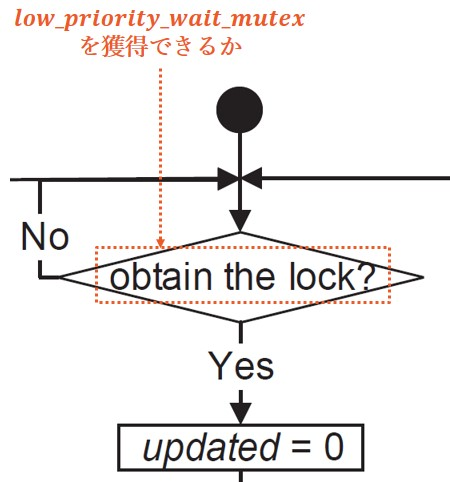
\includegraphics{figure/workflow1.jpg}
            }
        \end{column}
    \end{columns}
\end{frame}

\begin{frame}{reentrantとmutually exclusiveの違い}
    \begin{itemize}
        \item reentrant コールバックグループに属すwait\_set内のコールバックはいつでも選択できる
        \item 対照的に, mutually exclusive各コールバックグループにはフラグ \al{can\_be\_taken\_from} があり, そのグループに属すコールバックを選択して実行できるかどうかを示す
        \item グループのコールバックが実行のために選択されると, フラグは false に設定され, コールバックの終了後に true に設定される
        \item mutually exclusive コールバックグループに属すコールバックは,  can\_be\_taken\_from が true の場合にのみ選択できる
        \item それ以外の場合, スレッドはこのコールバックをスキップして次のコールバックに進む
    \end{itemize}
\end{frame}

\begin{frame}{can\_be\_taken\_fromによるワークフロー}
    \centering
    \vspace{\headerheight}
    \adjustbox{max width=\textwidth}{
        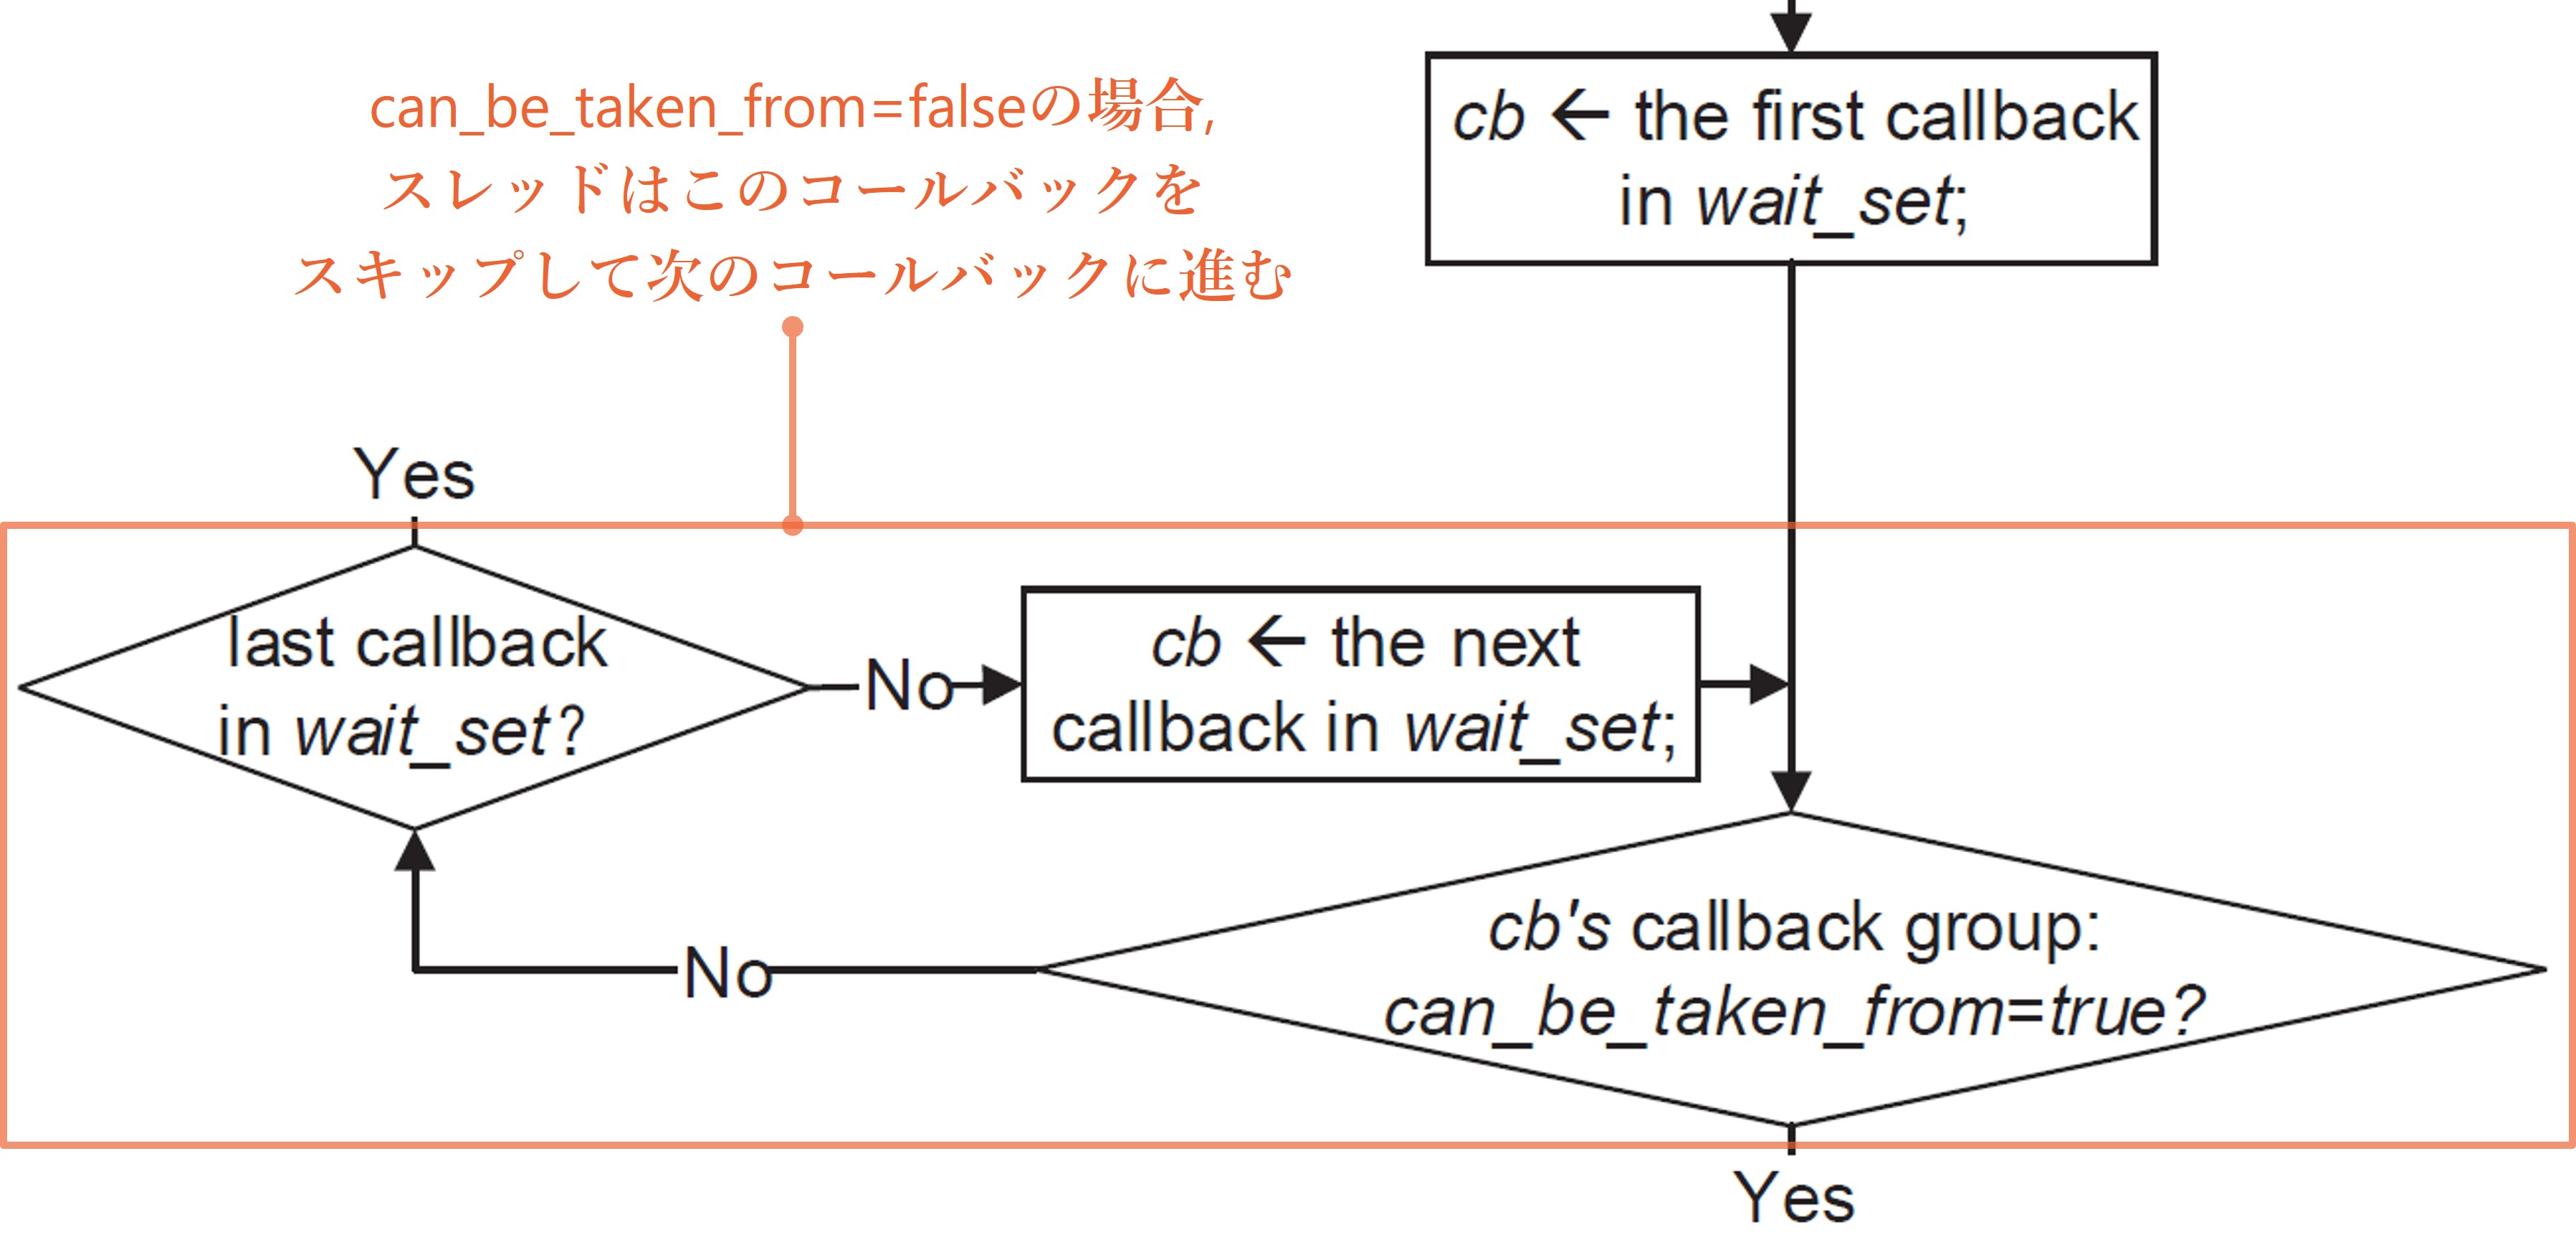
\includegraphics{figure/workflow2.jpg}
    }
\end{frame}

\begin{frame}{コールバック選択後}
    コールバックが正常に選択されると, スレッドは low\_priority\_wait\_mutex をリリースし, wait\_set からコールバックを削除する

    \centering
    \adjustbox{max width=\textwidth}{
        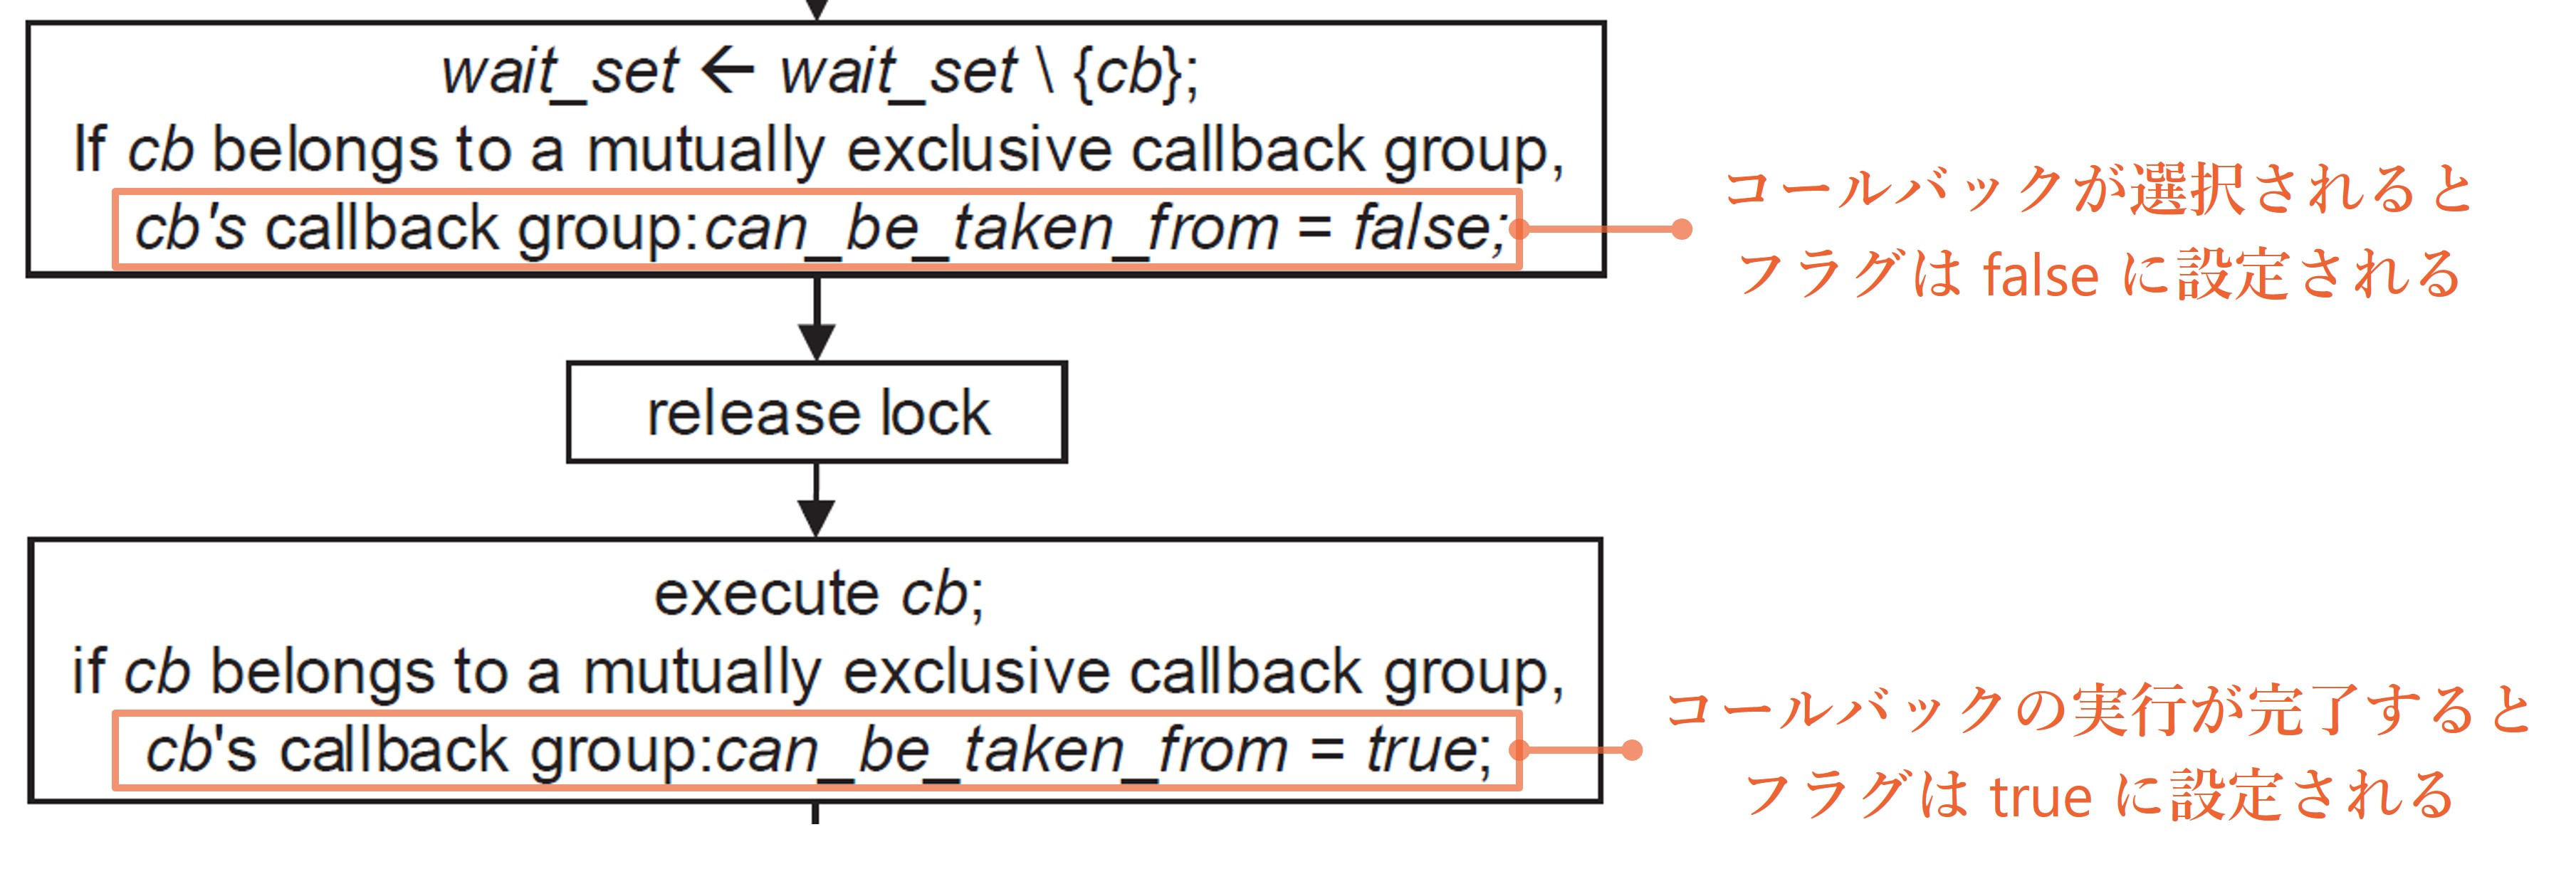
\includegraphics{figure/workflow3.jpg}
    }
\end{frame}

\begin{frame}{yield\_before\_execute}
    \setlength{\linewidth}{0.98\columnwidth}
    \begin{itemize}
        \item yield\_before\_execute の構成が false に設定されている場合, スレッドは選択されたコールバックの実行をすぐに開始する
        \item それ以外の場合, yield\_before\_execute が true に設定されている場合, スレッドは, 再度スケジュールされるまでプロセッサを OS に譲る
    \end{itemize}

    \assume{

        \begin{itemize}
            \item この作業では, 既定の構成 yield\_before\_execute $=$ false を考慮する
            \item コールバックは最も早く到着したメッセージでノンプリエンプティブに実行される
                  \begin{itemize}
                      \item ROS 2 では, 各コールバックには到着したメッセージをバッファリングするためのキューがあり, その深さはユーザによって指定される
                      \item キューが十分に大きく, メッセージが上書きされないと仮定する
                  \end{itemize}
        \end{itemize}
    }
\end{frame}

\begin{frame}{コールバックが選択できない場合}
    \vspace{\headerheight}
    \begin{itemize}
        \item すべてのカテゴリがチェックされ, 実行するコールバックを選択できない場合, スレッドは, wait\_set をリセットし, wait\_set を更新する
        \item can\_be\_taken\_from が true の場合にのみ, mutually exclusive コールバックグループからのコールバックを wait\_set に追加できる
    \end{itemize}

    \centering
    \adjustbox{max width=\textwidth, max height=0.6\textheight}{
        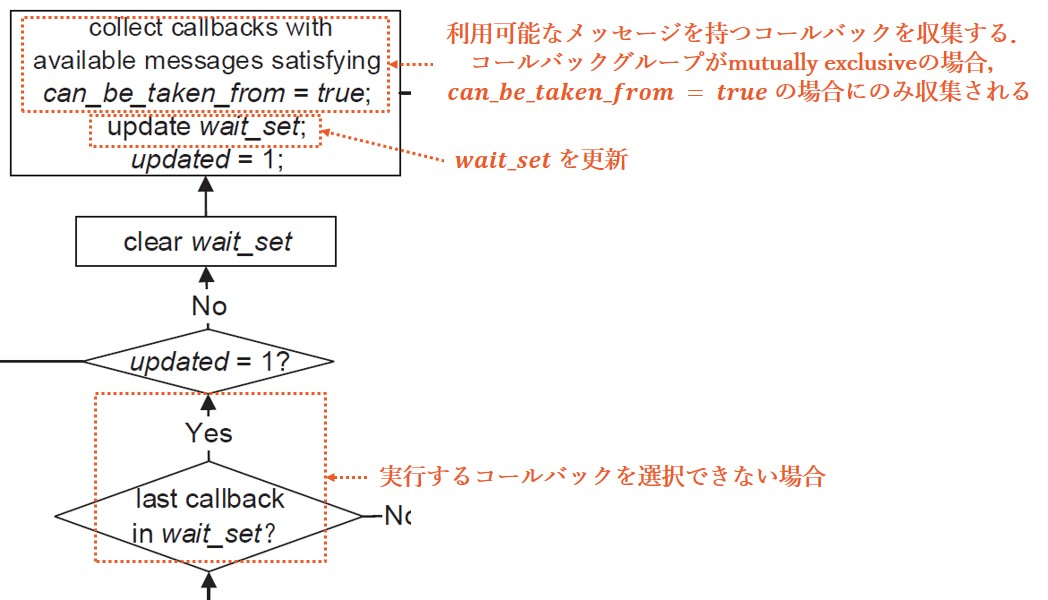
\includegraphics{figure/workflow4.jpg}
    }
\end{frame}

\begin{frame}{コールバックをwait\_setに追加できない場合}
    \begin{itemize}
        \item コールバックを wait\_set に追加できない場合, 頻繁なロックとロック解除によるオーバヘッドを回避するために, スレッドは, 新しいメッセージの到着によって通知されるか, 定義済みの最大ブロック時間に関してタイムアウトになるまでブロックされる
        \item それでも実行するコールバックが見つからない場合, スレッドはロックをリリースしてアイドル状態になる
    \end{itemize}
\end{frame}

\begin{frame}{コールバックをwait\_setに追加できない場合(ワークフロー)}
    \centering
    \vspace{\headerheight}
    \adjustbox{max width=0.9\textwidth}{
        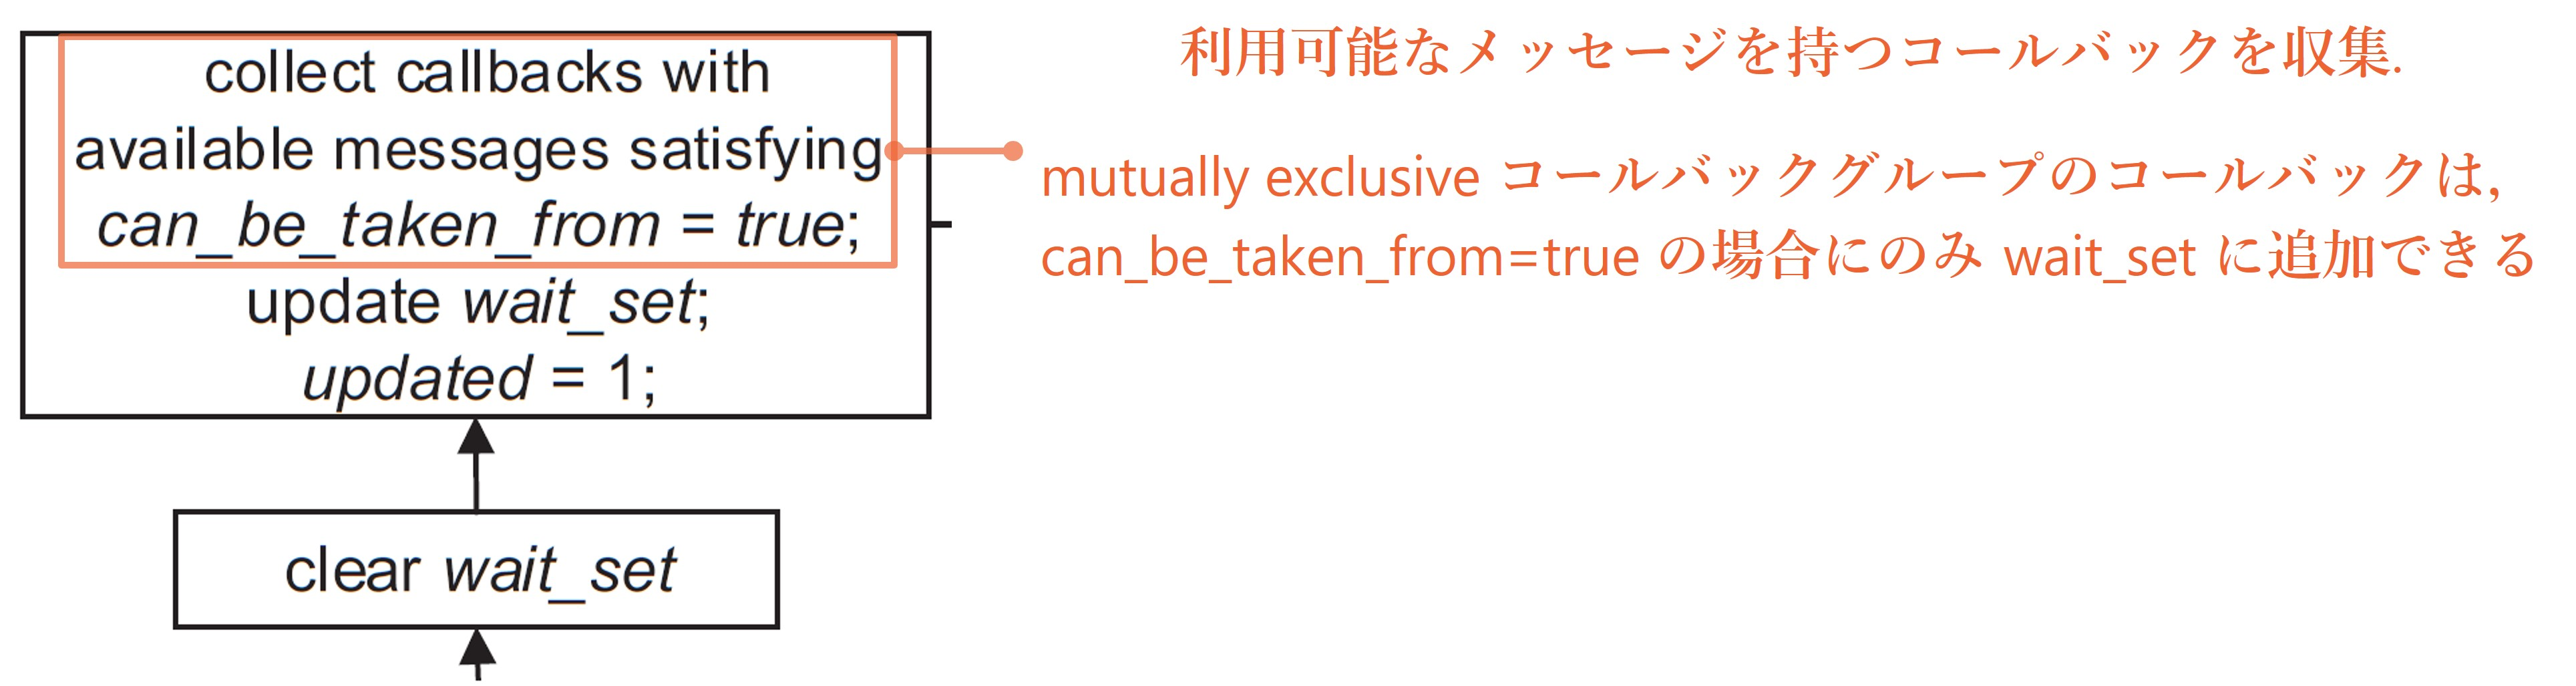
\includegraphics{figure/workflow5.jpg}
    }
\end{frame}
